\documentclass[sigconf]{acmart}

%%
%% \BibTeX command to typeset BibTeX logo in the docs
\AtBeginDocument{%
  \providecommand\BibTeX{{%
    Bib\TeX}}}

%% Rights management information.  This information is sent to you
%% when you complete the rights form.  These commands have SAMPLE
%% values in them; it is your responsibility as an author to replace
%% the commands and values with those provided to you when you
%% complete the rights form.
\copyrightyear{2023} 
\acmYear{2023} 
\setcopyright{rightsretained} 
\acmConference[UIST '23 Adjunct]{The 36th Annual ACM Symposium on User Interface Software and Technology}{October 29-November 1, 2023}{San Francisco, CA, USA}
\acmBooktitle{The 36th Annual ACM Symposium on User Interface Software and Technology (UIST '23 Adjunct), October 29-November 1, 2023, San Francisco, CA, USA}
\acmDOI{10.1145/3586182.3615800}
\acmISBN{979-8-4007-0096-5/23/10}

%%
%%  Uncomment \acmBooktitle if the title of the proceedings is different
%%  from ``Proceedings of ...''!
%%
%%\acmBooktitle{Woodstock '18: ACM Symposium on Neural Gaze Detection,
%%  June 03--05, 2018, Woodstock, NY}
% \acmPrice{15.00}
% \acmISBN{978-1-4503-6708-0/20/04}

%%
%% end of the preamble, start of the body of the document source.
\begin{document}

%%
%% The "title" command has an optional parameter,
%% allowing the author to define a "short title" to be used in page headers.
\title[Printed Circuit Board (PCB) Probe Tester (PCBPT) - a Compact Desktop System that Helps with \\ Automatic PCB Debugging]
{Printed Circuit Board (PCB) Probe Tester (PCBPT) - a Compact Desktop System that Helps with Automatic PCB Debugging}
% \title{Printed Circuit Board (PCB) Probe Tester (PCBPT)
% - a Compact Desktop System that Helps with Automatic PCB Debugging}

%%
%% The "author" command and its associated commands are used to define
%% the authors and their affiliations.
%% Of note is the shared affiliation of the first two authors, and the
%% "authornote" and "authornotemark" commands
%% used to denote shared contribution to the research.
\author{Fangzheng Liu}
\affiliation{%
  \institution{Responsive Environments, MIT Media Lab}
  \city{Cambridge}
  \country{USA}}
\email{fzliu@mit.edu}

\author{Joseph Paradiso}
\affiliation{%
  \institution{Responsive Environments, MIT Media Lab}
  \city{Cambridge}
  \country{USA}}
\email{joep@media.mit.edu}

\begin{abstract}
PCB debugging can be tricky. For example, if we want to use an oscilloscope to measure signals of interest in the PCB, we need to locate them in the schematic and select the appropriate pad for each signal on the PCB layout on which to put the oscilloscope probes. This process hence requires frequent switching between the schematics and the PCB layouts. Moreover, our hands may not be precise and stable enough to accurately place the probes on the pads without causing short circuits with adjacent pins, which can lead to further issues. Additionally, if multiple signals need to be tested, two hands will not be enough. Probe hook clips can be used, but this often necessitates the use of extension wires that must be soldered onto the targeted pads. To streamline the debugging process, we introduce the PCBPT (PCB Probing Tester). This innovative solution seamlessly bridges from schematic to test equipment by using a robotic probe and actuated board holder. By selecting signals of interest directly from a GUI, users can instantly monitor the output on an oscilloscope, significantly improving the effectiveness of the debugging process.
\end{abstract}

%%
%% The code below is generated by the tool at http://dl.acm.org/ccs.cfm.
%% Please copy and paste the code instead of the example below.
%%
\begin{CCSXML}
<ccs2012>
   <concept>
       <concept_id>10003120.10003121.10003129</concept_id>
       <concept_desc>Human-centered computing~Interactive systems and tools</concept_desc>
       <concept_significance>500</concept_significance>
       </concept>
 </ccs2012>
\end{CCSXML}

\ccsdesc[500]{Human-centered computing~Interactive systems and tools}
%%
%% Keywords. The author(s) should pick words that accurately describe
%% the work being presented. Separate the keywords with commas.
\keywords{compact desktop system, PCB, automatic debugging, in-circuit debugging}

% %% A "teaser" image appears between the author and affiliation
% %% information and the body of the document, and typically spans the
% %% page.
% \begin{teaserfigure}
%   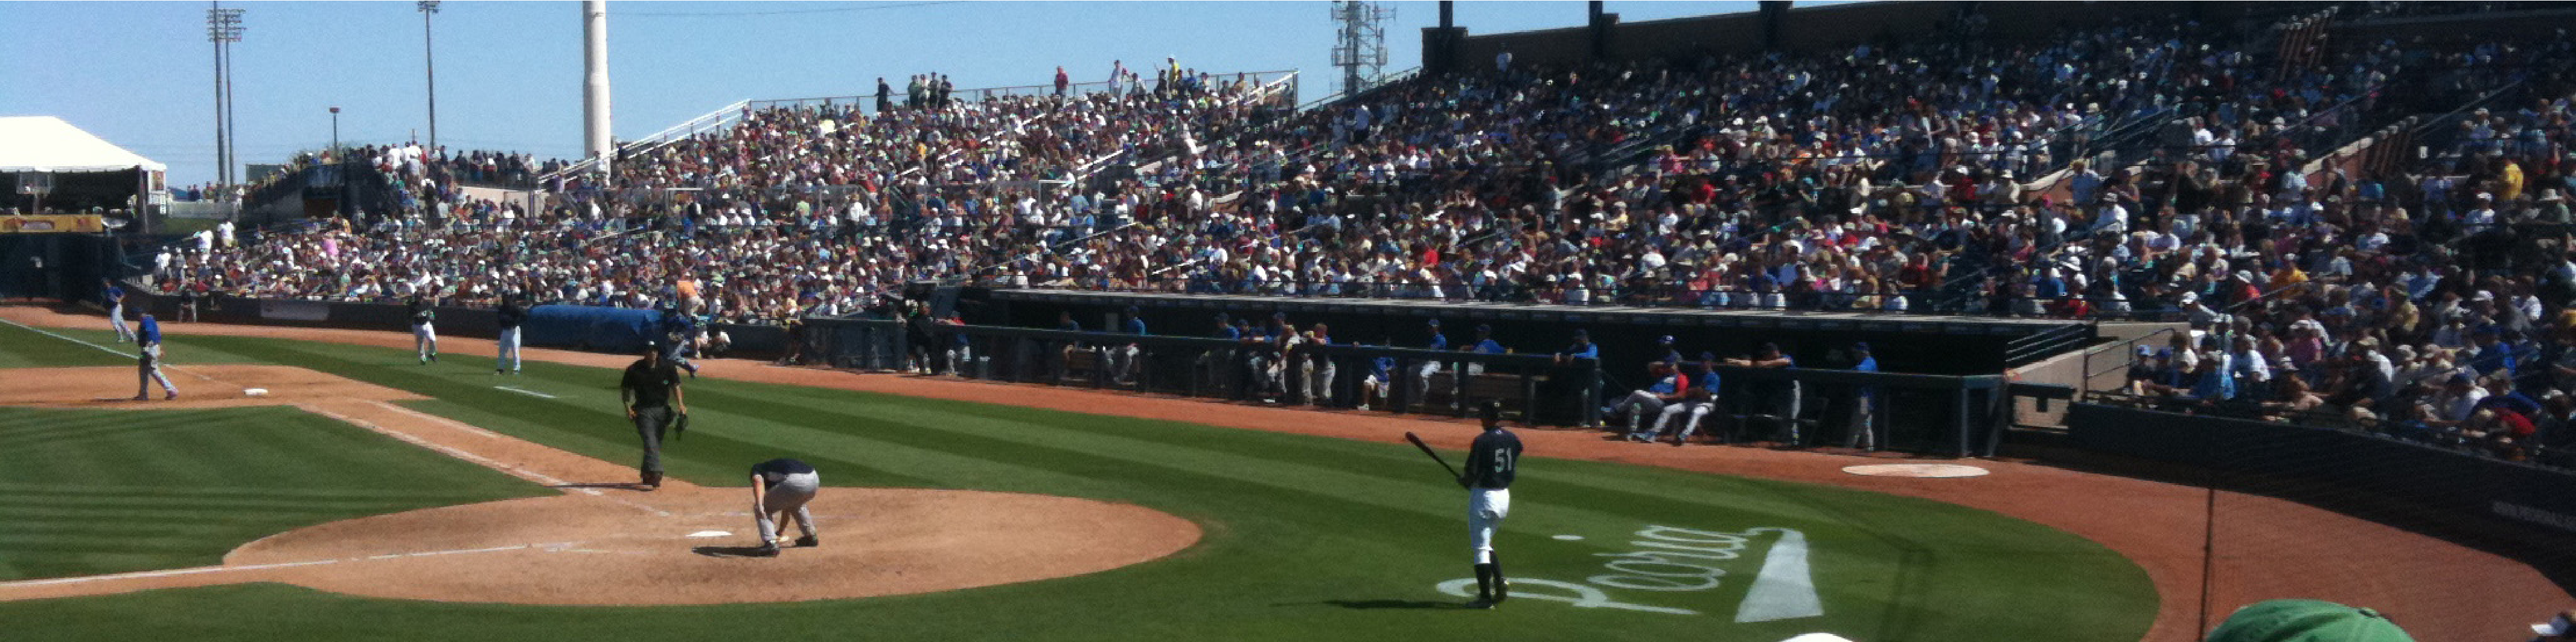
\includegraphics[width=\textwidth]{sampleteaser}
%   \caption{Seattle Mariners at Spring Training, 2010.}
%   \Description{Enjoying the baseball game from the third-base
%   seats. Ichiro Suzuki preparing to bat.}
%   \label{fig:teaser}
% \end{teaserfigure}

%%
%% This command processes the author and affiliation and title
%% information and builds the first part of the formatted document.
\maketitle

\section{Introduction}
To enhance the efficiency of debugging processes for hardware engineers and hobbyists, we have developed the PCBPT (PCB Probing Tester). Traditionally, for debugging the function of PCB, we need to measure signals of interest by using test equipment, such as an oscilloscope. This requires frequent switching between schematics and PCB layouts to identify signals of interest and select appropriate pads for probe placement. The manual probing method is prone to errors, such as short-circuiting adjacent pins and causing further issues \cite{automatic_compactpcbdebugging}. Additionally, when multiple signals need to be tested, the limitations of human hands become apparent. Although probe hook clips with extension wires are an alternative, they necessitate soldering on targeting pads, and when the size of the PCB is compact due to application limit, there is no space for extra test points pads for debugging.

A bed-of-nails jig is an alternative. However, it requires the consuming design and production of a jig for each specific PCB design, rendering it inefficient for even minor component position changes since it requires a redesign and production of the jig. Commercial flying probe testers are expensive and bulky, making them unsuitable for hobbyists and small companies.

The PCBPT is a compact desktop tool, and by leveraging the information contained in the PCB layout, and eliminating the need for manual probing, the PCBPT revolutionizes the way debugging is conducted and allows users to select signals of interest and immediately view the output on an oscilloscope. This streamlined workflow significantly enhances the effectiveness of debugging. With the PCBPT, engineers can efficiently interact with their designs during the debugging process.

% It empowers hardware engineers and hobbyists to achieve precise and fast diagnostics without the limitations of traditional methods or the cost and size constraints associated with commercial solutions.

\section{System structure}
The PCBPT works with PCB designed by EAGLE — an electronic design automation (EDA) software for PCB design. The entire system comprises two components: the Data Processing Program and the PCBPT Probe Machine, as illustrated in Fig.\ref{PCBPT_structure}.

\begin{figure}[h]
  \centering
  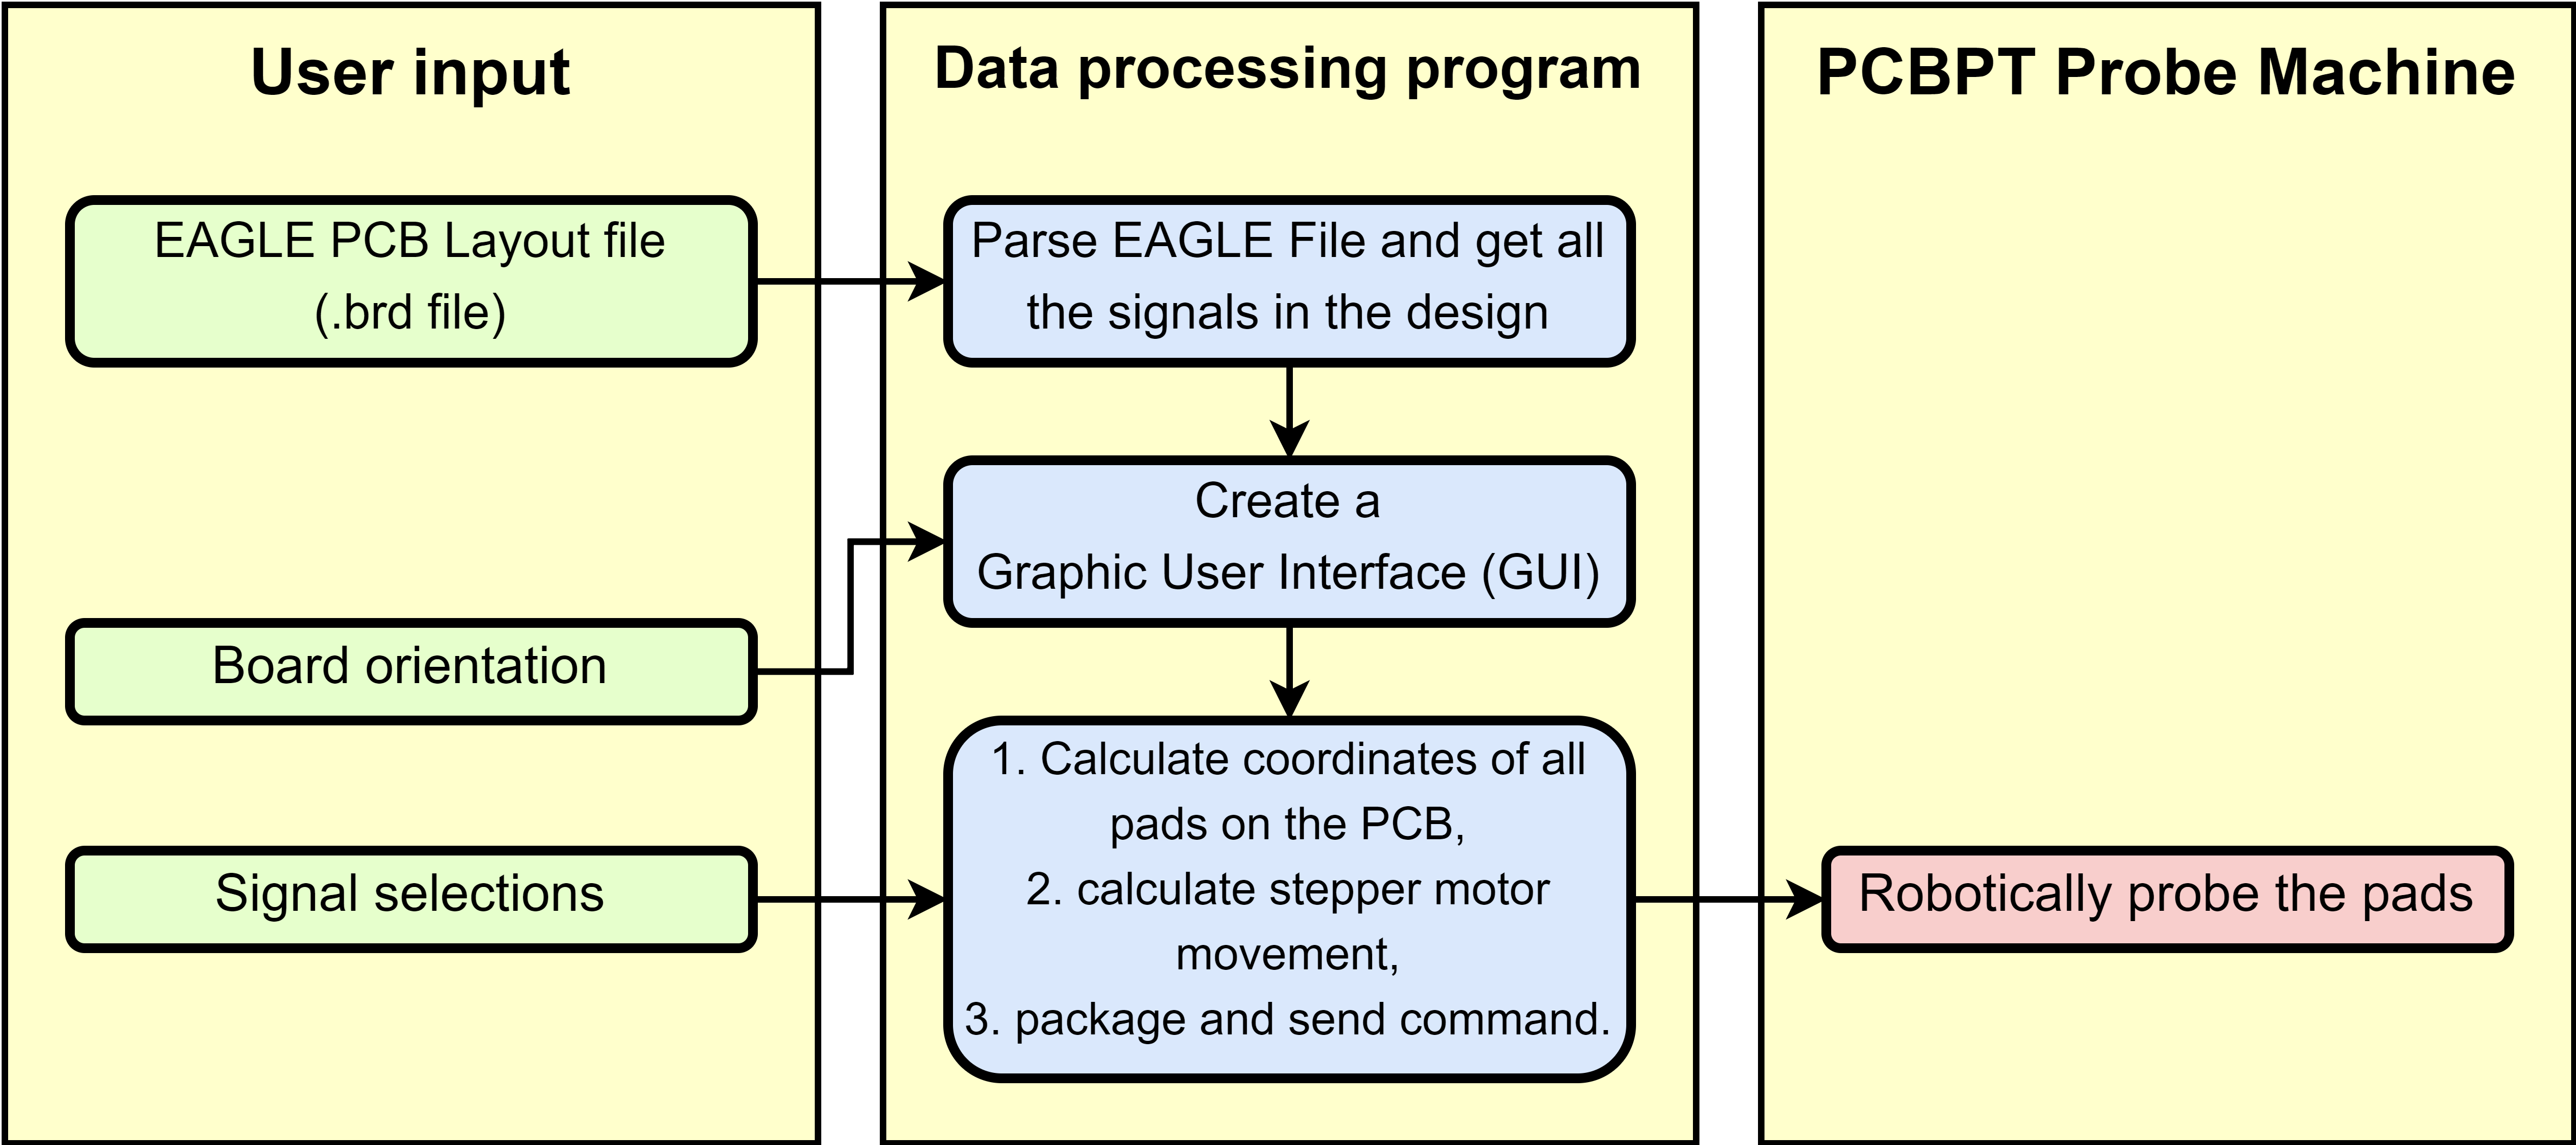
\includegraphics[width=\linewidth]{PCBPT_structure.png}
  \caption{The PCBPT system structure}
  \label{PCBPT_structure}
  \Description{Structure of the PCBPT system. The system accepts Users input, including EAGLE design files, board orientation and signals to be measured. A program parses the data input and calculates the coordinates of all pads on the PCB. Upon signals selections, the program controls the machine to probe the corresponding pads.}
\end{figure}

\subsection{Data Processing Program}
The Data Processing Program is written in Python and performs several key functions, such as accepting and parsing user input, including the EAGLE PCB layout file (.brd), and the orientation of the tested board on the PCBPT Probe machine. Additionally, it creates a user-friendly GUI for signal selection, calculates PCB pad coordinates, and controls probe movements on the machine.
The EAGLE PCB layout design file is encoded in XML format, making it readily parseable in Python. Upon importing the $.brd$ file, the program extracts and stores comprehensive information about all components and signals within the PCB design. It then generates a user-friendly GUI that displays a list of all signals for selection. Through the GUI, the user can choose specific signals of interest. Subsequently, the program automatically determines the appropriate pads, based on the size of the pads and type of the components for the selected signals and calculates their corresponding coordinates. A command is then issued to the machine to initiate the probing process on the identified pads. The subsequent section will provide a detailed explanation of the coordinate calculation method.

The program generates a GUI (as shown in Fig.\ref{GUI}) to facilitate the user's interaction. As an example, we select the Adafruit LIS3DH breakout board \cite{Adafruit_LIS3DH} to demonstrate its functionality within the GUI.

\begin{figure}[h]
  \centering
  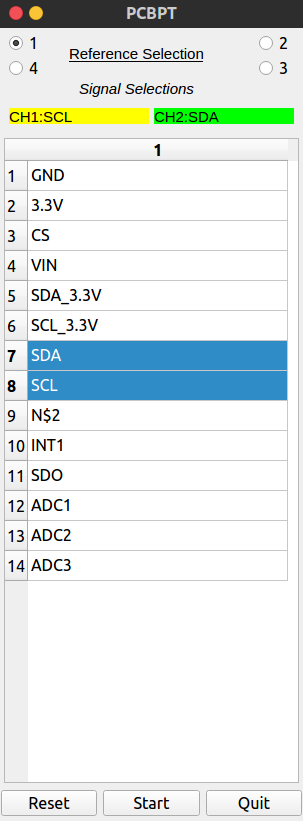
\includegraphics[width=0.17\textwidth]{gui.png}
  \caption{The GUI for the user to select signals to be measured.}
  \label{GUI}
  \Description{The GUI of the PCBPT. It shows the list of signals in the PCB design, and users can select the desired signals to be measured.}
\end{figure}

\subsection{PCBPT Probe Machine}
The PCBPT Probe Machine is a compact ($35.0cm \times 12.5cm \times 24.8cm$) 3D-printed CNC machine with two probes, as shown in Fig.\ref{machine}. The PCB to be tested is positioned and secured on the machine platform.

\begin{figure}[h]
  \centering
  \includegraphics[width=\linewidth]{pcbpt_probe_machine.jpg}
  \caption{PCBPT Probe Machine}
  \label{machine}
  \Description{The PCBPT machine --- a CNC machine with two gantries, and each gantry has a probe.}
\end{figure}

The machine utilizes stepper motors for actuation in the XY axis, while tiny linear servos drive the two probes in the Z axis. The electronic system structure of the machine is illustrated in Figure \ref{electronics_structure}. To facilitate the robotic probing of targeted pads, an Arduino Mega2560 board is employed. It receives commands from the Data Processing Program and controls the four steppers for XY-axis movement, as well as the servos for Z-axis movement to probe the targeted pads.

\begin{figure}[h]
  \centering
  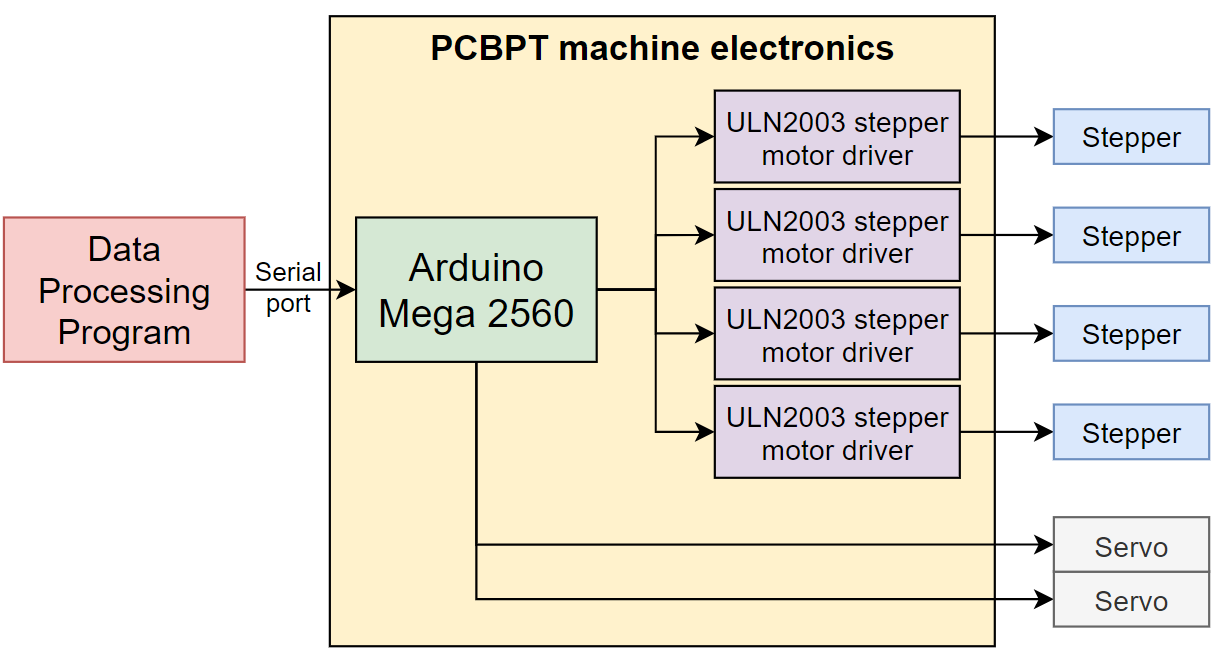
\includegraphics[width=\linewidth]{electronics_structure.png}
  \caption{PCBPT Probe Machine electronics system}
  \label{electronics_structure}
  \Description{The PCBPT electronics system. The core part is an Arduino Mega 2560 board which is connected to four stepper motor driver modules.}
\end{figure}

Prior to utilization, the machine undergoes calibration to establish the correlation between the stepper motor's steps and the actual distance covered during movement.

\section{Workflow}
This section outlines the workflow for utilizing the PCBPT in automating the process of PCB debugging.

\subsection{Calibration}
To align the coordinates of all pads in the PCB design with the machine's coordinate system, the user must first specify the board's orientation on the holder relative to the PCB layout design through the GUI. Currently, the machine only supports square-shaped PCBs, allowing orientations of $0^{\circ}$, $90^{\circ}$, $180^{\circ}$, and $270^{\circ}$. After selecting an orientation, the user manually controls the machine to probe a chosen pad and records the corresponding movements. By incorporating the orientation and the steps bias, the program utilizes a rotation equation \cite{rotation_equation} to calculate the coordinates of all pads in the machine's coordinate system.

The current calibration approach is straightforward and will benefit from enhancements (e.g., using a camera and image processing for the automatic board, components, and pad detections\cite{inspect_ar}) to improve its effectiveness and accuracy.

\subsection{Probe}
Upon powering on, the machine will automatically position the two probes to their start positions. Once the user selects the desired signals for measurement from the GUI and clicks the "Start" button, the program will send a digital command to the machine that will specify the direction and the number of steps each motor should move. Subsequently, the machine will control the probes to accurately and automatically contact the corresponding pads on the PCB. To facilitate real-time signal analysis, each probe can be connected to a separate channel of an oscilloscope, which instantly visualizes the waveform of the selected signals, as shown in Fig.\ref{result}. In this measurement, we use the Adafruit LIS3DH breakout board as an example and measured the $I^2C$ signals.

\begin{figure}[h]
  \centering
  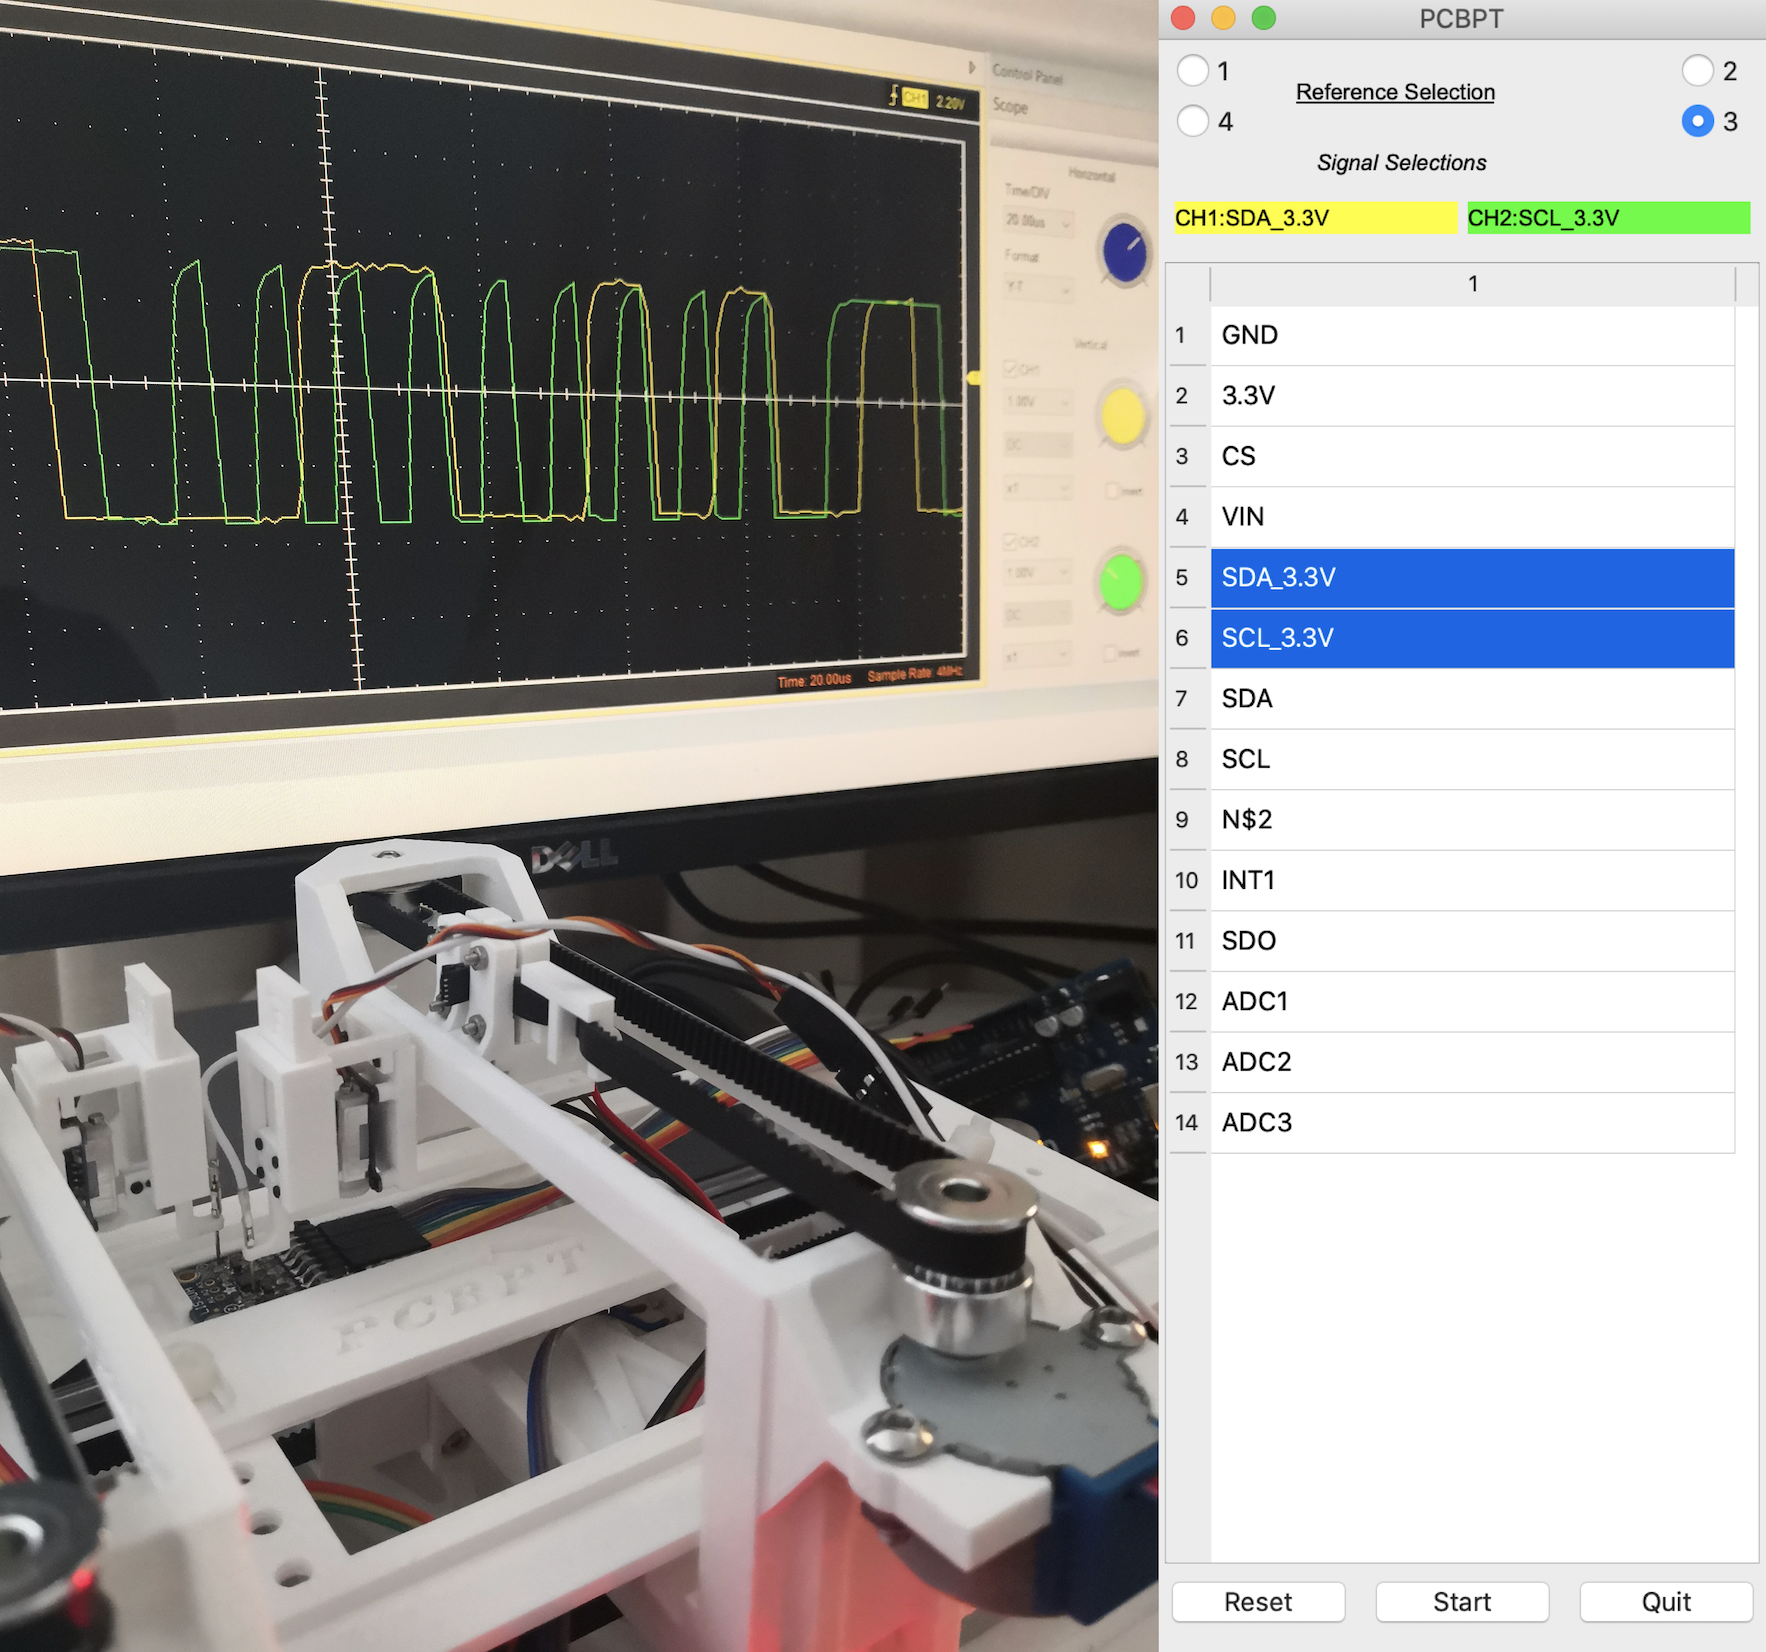
\includegraphics[width=\linewidth]{result.png}
  \caption{PCBPT automatically probes the desired pads and an oscilloscope visualizes the signals.}
  \label{result}
  \Description{The PCBPT helps with automatic probing the I2C signal on a small PCB.}
\end{figure}

\section{Conclusion}
The PCBPT system introduces an innovative approach by directly connecting the PCB schematic with the signals output, bridging the gap between design and real-world measurements. However, there are identifiable limitations within the current design, For instance, the system currently supports testing only one side of the PCB, employs only two probes, and utilizes a calibration approach that lacks efficiency. Additionally, the dimensions of the PCBs that can be tested are currently restricted to $50mm \times 70mm \times 4mm$. We hope that through further enhancements, this system could be a useful tool for future engineers and hardware hobbyists.  Improvements could include a camera on the probe and allowing the probe to tilt for use in cases where a pad can’t easily be accessed only by vertical movement and/or component shape inhibits easy access to a pad.  It would also be possible to combine simulation or cached data with the signals, displaying for example expected voltage levels and waveforms with the actual data, as used in \cite{boardlab}.


%%
%% The next two lines define the bibliography style to be used, and
%% the bibliography file.
\bibliographystyle{ACM-Reference-Format}
\bibliography{sample-base}


%%
%% If your work has an appendix, this is the place to put it.
\appendix

\end{document}
\endinput
%%
%% End of file `sample-lualatex.tex'.
